\section{Risikoanalyse}
In einem Projekt können immer wieder Probleme auftreten. In diesem Kapitel wird sich mit diesem Thema auseinandergesetzt und gezeigt, mit welchen Methoden auf die unterschiedlichen Eventualitäten reagiert werden kann.
Nachfolgend sind mögliche Risiken tabellarisch aufgelistet, sowie Maßnahmen um diese zu vermindern.\\
% Table generated by Excel2LaTeX from sheet 'Tabelle1'
\begin{table}[htbp]
  \centering
  \caption{Risiken und Massnahmen}
    \begin{tabular}{|r|r|l|l|}
    \toprule
    \multicolumn{1}{|l}{\textbf{Risiken}} & \multicolumn{1}{r}{} &       & \textbf{Massnahmen} \\
    \hline
    \multicolumn{1}{|l|}{Nr.} & \multicolumn{1}{l|}{Kategorien} & Identifikation &  \\
    \hline
    1     & \multicolumn{1}{l|}{Student} & Ausfall wegen Krankheit & Keine spezielle Massnahme \\
\cline{1-1}\cline{3-4}    2     &       & Studiumsabbruch & Niemand hat dies vor \\
\cline{1-1}\cline{3-4}    3     &       & Konflikte im Team & Klare Kommunikation \\
\cline{1-1}\cline{3-4}    4     &       & Fachliche Überforderung & Hilfe suchen bei Dozenten \\
\cline{1-1}\cline{3-4}    5     &       & Terminliche Überforderung & Vorausschauende Zeitplanung \\
    \hline
    6     & \multicolumn{1}{l|}{Daten} & Notebook kaputt & Backup, Ersatznotebook \\
\cline{1-1}\cline{3-4}    7     &       & versehentliches löschen & Backup \\
    \hline
    8     & \multicolumn{1}{l|}{Sonstiges} & Teile werden nicht geliefert & Woanders bestellen/Express Lieferung\\
\cline{1-1}\cline{3-4}    9     &       & Kein eigener Arbeitsplatz & Platz im Studentenlabor \\
    \bottomrule
    \end{tabular}%
  \label{tab:RisikenUndMassnahmen}%
\end{table}%

Tabelle \ref{tab:RisikenUndMassnahmen} zeigt eine nummerierte Auflisten von möglichen Risiken und Massnahmen um diese zu vermindern. Eine Heat Map wird estellt, welche die Risiken nach Auswirkung und Eintrittswahrscheinlichkeit graphisch darstellt. Mit einem Pfeil wird die neue Position des Risikos mit greifender Massnahme angedeutet. So soll ein Überblick über mögliche Risiken und deren Potenzial gegeben werden.\\

\begin{figure}[h]
\centering
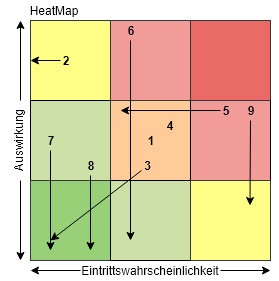
\includegraphics[scale=0.65]{graphics/HeatMap.PNG}
\caption{Heat Map}
\label{fig:HeatMap}
\end{figure}

Abbildung \ref{fig:HeatMap} gibt einen Überblick über mögliche Risiken und deren Potenzial, wobei die Nummern gemäss Tabelle \ref{tab:RisikenUndMassnahmen} definiert sind. Es ist ersichtlich, dass einige Massnahmen gewisse Risiken stark minimieren. Die grössten Risiken sind der Ausfall wegen Krankheit und fachliche sowie terminliche Überforderung. Auf diese Risiken soll während des Projekts speziell geachtet werden, um eine frühzeitige Erkennung zu gewährleisten.\\ 
